\documentclass[a4paper,12pt]{article} % тип документа


\usepackage[T2A]{fontenc}			% кодировка
\usepackage[utf8]{inputenc}			% кодировка исходного текста
\usepackage[english,russian]{babel}	% локализация и переносы
\usepackage{amsfonts,longtable}
\usepackage[pdftex]{graphics}
\usepackage{tikz}
\usepackage{mathrsfs}
\usepackage{wrapfig}
\usepackage{array}
\usepackage[american,siunitx,smartlabels]{circuitikz} 
\usepackage{amsmath,amsfonts,amssymb,amsthm,mathtools} 
\usepackage{wasysym}

\title{Лабораторная работа 1.1.4 по курсу \\ "Общая физика"  \\ 
\vspace{0.2cm}
\vspace{4.5cm}
 \LARGE{\textbf{Измерение интенсивности радиационного фона}}\vspace{5.5cm}}
\date{05.10.2018}
\usepackage{tikz}
\author{\vspace{0.2cm}Баринов Леонид}
\begin{document}
\maketitle
\newpage
\section{Аннотация}
В данной работе измеряется число частиц, проходящих через счетчик за 10 и 40 секунд. Выбор времен измерения связан с желанием продемнострировать, что при большем времени лучше выполняется нормальное распределние измеряемых величин и гистограмма более симметрична, чем при малых временах.
\section{Теоретические сведения}
Поток космических частиц, которые составляют значительную часть радиационного фона, изменяется со временем случайным обазом. Харатеристиками этой величины в целом является ее среднее значение и среднеквадратичное отклонение от этого среднего.

Плотность потка частиц измеряется количеством частиц, проходящих за 1 секунду через площадку в $1\text{см}^2$. 

Среднеквадратичная ошибка числа отсчетов, измеренного за некоторый интервал времени, равна корню квадратному из среднего числа отсчетов за тот же интервал: $\sigma = \sqrt{n_0}$. Однако истенное среднее значение измеряемой величины неизвестно. Поэтому в формулу для определения стандартной ошибки отдельного измерения приходится подставлять не истинное среднее значение $n_0$, а измерение значение $n$:
\begin{equation}
\label{1}
\sigma = \sqrt{n}
\end{equation}
Формула (\ref{1}) показывает, что, как правило (с вероятностью $68\%$), измеренное число частиц $n$ отличается от искомого среднего не более чем $\sqrt{n}$. Результат измерений записывается так:
\begin{equation}
\label{2}
n_0 = n \pm \sqrt{n}
\end{equation}
Мы провели серию из $N$ измерений, в результате которых получены числа частиц $n_1, n_2, ..., n_N$. При $N$  измерениях среднее значение числа сосчитанных за одно измерение частиц равно:
\begin{equation}
\label{3}
\overline{n} = \frac{1}{N}\sum_{i=1}^{N}n_i
\end{equation}
Стандартную ошибку отдельного измерения можно оценить по формуле:
\begin{equation}
\label{4}
\sigma_\text{отд} = \sqrt{\frac{1}{N}\sum_{i=1}^{N}(n_i-\overline{n})^2}
\end{equation}
В сооветствии с формулой (\ref{1}) следует ожидать, что эта ошибка будет близка к $\sqrt{n_i}$, т. е. $\sigma_\text{отд}\approx\sigma_i=\sqrt{n_i}$. 
Ближе всего к значению $\sigma_\text{отд}$, определнному по формуле (\ref{4}), лежит, конечно, величина  $\sqrt{\overline{n}}$, т. е.
\begin{equation}
\label{5}
\sigma_\text{отд} \approx \sqrt{\overline{n}}
\end{equation}
Теория вероятностей показывает, что стандартная ошибка отклонения $\overline{n}$ от $n_0$ может быть определена по формуле:
\begin{equation}
\label{6}
\sigma_\text{отд} = \sqrt{\frac{1}{N}\sum_{i=1}^{N}(n_i-\overline{n})^2} = \frac{\sigma_\text{отд}}{\sqrt{N}}
\end{equation}
Для рассмотренной серии из $N$ измерений по 10 с относительная ошибка отдельного измерения (т. е. ожидаемое отличие любого из $n_i$ от $n_0$)
\begin{equation}
\label{7}
\varepsilon_\text{отд} = \frac{\sigma_\text{отд}}{n_i} \approx \frac{1}{\sqrt{n_i}}
\end{equation}
Аналогичным образом определяется относительная ошибка в определении среднего по всем измерениям значения $\overline{n}$:
\begin{equation}
\label{8}
\varepsilon_{\overline{n}} = \frac{\sigma_{\overline{n}}}{\overline{n}} = \frac{\sigma_\text{отд}}{\overline{n} \sqrt{N}} \approx \frac{1}{\sqrt{\overline{n}N}}
\end{equation}
Доля случаев $\omega_n$, характеризующая вероятность получить $n$ отсчетов, определяется по формуле:
\begin{equation}
\label{9}
\omega_n = \frac{\text{число случаев с отсчетом }n}{\text{полное число измерений }(N)}
\end{equation}
\section{Оборудование и инструментальные погрешности}
Обноружить космические лучи и измерить их интенсивность можно по ионизации, которую они производят. Для этого используется специальный прибор - счетчик Гейгера-Мюллера. Счетчик представляет собой наполненный газом сосуд с двумя электродами. Существует несколько типов таких счетчиков. Используемый в данной работе (СТС-6) представляет собой тонкостенный металлический цилиндр, который является одним из электродов (катодом). Другим электродом (анодом) является тонкая нить, натянутая вдоль оси цилиндра. Чтобы счетчик работал в режиме счета частиц, на электроды необходимо подать напряжение 400В. Частицы космических лучей ионизируют газ, которым наполнен счетчик, а также выбивают электроны из его стенок. Образовавшиеся электроны, ускоряясь в сильном поле между электродами счетчика, соударяются с молекулами газа и выбивают из них новые вторичные электроны. Эти электроны ускоряются электрическим полем и затем ионизируют молекулы газа. В результате образуется целая лавина электронов, и через счетчик резко увеличивается ток. На рис. 1 приведена схема включения счетчика.

\begin{wrapfigure}{r}{4cm}
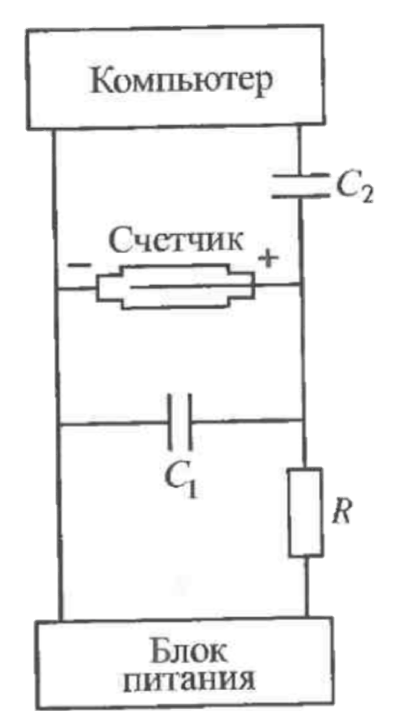
\includegraphics[width=0.3\textwidth]{3}
\caption{Cхема включения счетчика}
\end{wrapfigure}Постоянное напряжение подается на счетчик от блока питания через сопротивление $R$. В исходном состоянии электроды СТС-6 и конденсатор $C_1$ заряжены до напржяения 400 В, так как сопротивление резистора $R$ много меньше сопротивлений утечки СТС-6 и конденсатора $C_1$. Разделительный конденсатор $C_2$ не пропускает постоянное напряжение источника питания в интерфейсные схемы компьютера.

При возниковении тока через счетчик заряд на СТС-6 и конденсаторе $C_1$ обеспечивает развитие электронной лавины на короткое время. В процессе разряда энергия поступает от заряженного коденсатора $C_1$, подсоединенного параллельно счетчику. Разряд в счетчике прекратится, когда напряжение на счетчике уменьшиться до значения, при котором разность потенциалов внутри счетчика на длине свободного пробега электрона не превышает потенциала ионизации. За время порядка нескольких $RC_1$ схема приходит в исходное состояние. При этом через конденсатор $C_2$ в электронную схему интерфейса компьютера будет передан короткий импульс.

Емкость конденсатора $C_1$ не должна быть ни слишком малой, ни слишком большой. Запасенной в конденсаторе энергии должно хватить на создание лавинного процесса, но вместе с тем время зарядки конденсатора от блока питания ($\tau \sim RC_1$), называемое мертвым временем счетчика, не должно быть слишком большим, так как в течение этого времени счетчик не может регистрировать частицы (обычно мертвое время составляет несколько микросекунд). В нашей установке этим условиям вполне удовлетворяет емкость самого счетчика, и конденсатор $C_1$ отсутствует.

Сопротивление резистора $R$ также не должно быть ни слишком большим (это увеличивает мертвое время счетчика), ни слишком малым, чтобы конденсатор за время разряда не успевал существенно зарядиться и лавина гасла. Обычно $R \sim 1\text{МОм}$.

Число зарегестрированных частиц зависит от времени измерения, размеров счетчика, состава газа и давления в нем, а также от материала, из которого сделаны стенки счетчика. Значительную часть регистрируемых частиц составляет естественный радиоактивный фон.

Оценки показывают, что погрешности измерений потока частиц с помощью счетчика Гейгера-Мюллераи малы по сравнению с изменениями самого потока или, как говорят, с флуктуациями потока. Погрешности измерений определяются в основном временем, в течение которого восстанавливаются нормальные условия в счетчике после прохождения каждой частицы и срабатывания счетчика. Это время называется временем разрешения. Размеры счетчика должны быть такими, чтобы время между попаданиями частиц в счетчик было больше времени разрешения.

В работе для организации процесса измерения плотности космических лучей и процессе обработки эксперементальных данных используется специально разработанная компьютерная программа. При проведении эксперимента программа позволяет посмотреть, как во время эксперимента меняется сама сама исследуемая величина, ее среднее значение, стандартное отклонение (погрешность).

\section{Результаты измерений и обработка данных}
Измеряем плотность потока космического излучения за 10 секунд. На компьютере провдем обработку данных. Результаты приведены в Таблице 1 и Таблице 2
\newpage
\begin{table}[h]
\centering
\caption{Число срабатываний счетчика за 20с}
\label{table 1}
\renewcommand{\tabcolsep}{2mm}
\begin{tabular}{|c|l|l|l|l|l|l|l|l|l|l|}
\hline
№ опыта & \multicolumn{1}{c|}{1} & \multicolumn{1}{c|}{2} & \multicolumn{1}{c|}{3} & \multicolumn{1}{c|}{4} & \multicolumn{1}{c|}{5} & \multicolumn{1}{c|}{6} & \multicolumn{1}{c|}{7} & \multicolumn{1}{c|}{8} & \multicolumn{1}{c|}{9} & \multicolumn{1}{c|}{10} \\ \hline
0&31 & 24 & 35 & 33 & 25 & 41 & 32 & 27 & 33 & 27 \\ \hline
1&33 & 32 & 41 & 28 & 30 & 25 & 21 & 31 & 32 & 22 \\ \hline
2&21 & 39 & 33 & 29 & 17 & 25 & 32 & 28 & 35 & 25 \\ \hline
3&24 & 26 & 24 & 33 & 21 & 28 & 23 & 20 & 34 & 31 \\ \hline
4&22 & 23 & 30 & 23 & 25 & 25 & 36 & 23 & 28 & 23 \\ \hline
5&29 & 28 & 24 & 20 & 37 & 29 & 32 & 30 & 34 & 31 \\ \hline
6&27 & 26 & 31 & 21 & 28 & 29 & 25 & 38 & 33 & 25 \\ \hline
7&22 & 23 & 23 & 23 & 30 & 30 & 20 & 34 & 24 & 27 \\ \hline
8&20 & 29 & 22 & 17 & 35 & 19 & 28 & 33 & 28 & 24 \\ \hline
9&28 & 31 & 29 & 29 & 32 & 38 & 33 & 39 & 41 & 32 \\ \hline
10&27 & 40 & 38 & 26 & 23 & 29 & 27 & 17 & 28 & 26 \\ \hline
11&27 & 25 & 30 & 18 & 25 & 25 & 17 & 32 & 37 & 30 \\ \hline
12&30 & 22 & 22 & 33 & 39 & 30 & 31 & 22 & 33 & 25 \\ \hline
13&26 & 25 & 27 & 30 & 32 & 26 & 35 & 29 & 37 & 31 \\ \hline
14&25 & 20 & 24 & 28 & 31 & 26 & 35 & 30 & 26 & 29 \\ \hline
15&33 & 19 & 27 & 29 & 24 & 15 & 31 & 30 & 20 & 33 \\ \hline
16&32 & 30 & 26 & 31 & 23 & 30 & 25 & 37 & 23 & 22 \\ \hline
17&25 & 28 & 27 & 27 & 22 & 25 & 25 & 23 & 35 & 17 \\ \hline
18&29 & 34 & 29 & 32 & 27 & 36 & 27 & 29 & 34 & 27 \\ \hline
19&23 & 28 & 17 & 32 & 32 & 25 & 21 & 32 & 27 & 30 \\ \hline
\end{tabular}
\end{table}

Разбиваем результаты измерений из Таблицу 1 в порядке их получения на группы по 2, что соответстует проведению $N_2 = 100$ измерений числа частиц за интервал времени, равный 40 с. Результаты сведем в Таблицу 3

Представим результаты последнего распределения в виде, удобном для построения гистограммы (Таблица 4). Гистограммы распределений среднего числа отсчетов за 10 и 40 с строим на одном графике (Рис. 2). При этом для второго распределения цену деления по оси абсцисс увеличиваем в 4 раза, чтобы положения максимумов распределений совпадали.

Используя формулу (3), определим среднее число срабатываний счетчика за 10 с:
\[\overline{n}_1 = \frac{1}{N_1}\sum_{i=1}^{N_1}n_i = \frac{5600}{400}=14\]
\newpage
\begin{table}[h]
\centering
\caption{Данные для построения гистограммы распределения числа срабатываний счетчика за 10с}
\label{table 2}
\begin{tabular}{|c|c|c|c|c|c|c|}
\hline
Число импульсов $n_i$ & 5 & 6 & 7 & 8 & 9 & 10 \\ \hline
Число случаев   &  2 & 5  & 10  & 7  & 15  & 24  \\ \hline
Доля случаев $\omega_n$   & 0,005  & 0,0125  & 0,025  & 0,0175  & 0,0375  & 0,06  \\ \hline\hline
Число импульсов $n_i$ & 11& 12 & 13 & 14 &15 & 16 \\ \hline
Число случаев   & 42 & 42  &39   & 45  & 34  & 38  \\ \hline
Доля случаев $\omega_n$   & 0,105  & 0,105  & 0,0975  & 0,1125  & 0,085  &0,095   \\ \hline\hline
Число импульсов $n_i$ & 17 & 18 & 19 & 20 &21 & 22 \\ \hline
Число случаев   &  32 & 19  & 14  & 12  & 9  & 3  \\ \hline
Доля случаев $\omega_n$   & 0,08  & 0,0475  & 0,035  & 0,03  & 0,0225  & 0,0075  \\ \hline
Число импульсов $n_i$ &23 & 24 & 25 & 26 &27 & 28 \\ \hline
Число случаев   &  4 & 2  &1   & 1  & 0  &0   \\ \hline
Доля случаев $\omega_n$   & 0,01  & 0,005  & 0,0025  & 0,0025  & 0  & 0  \\ \hline
\end{tabular}
\end{table}

Найдем среднеквадратичную ошибку отдельного измерения по формуле (4):
\[\sigma_1 = \sqrt{\frac{1}{N_1}\sum_{i=1}^{N_1}(n_i-\overline{n}_1)^2}=\sqrt{\frac{5722}{400}} \approx 3,78\]

Убедимся в справедливости формулы (5):
\[
\begin{aligned}
\sigma_1 \approx \sqrt{\overline{n}_1}; &  & 3,78 \approx \sqrt{14} = 3,74\\
\end{aligned}
\]

Определим долю случав, когда отклонения от среднего значения не превышают $\sigma_1$, $2\sigma_1$, и сравним с теоретическими оценками (Таблица 5).

Используя формулу (3), определим среднее число импульсов счетчика за 40 с:
\[\overline{n}_2 = \frac{1}{N_2}\sum_{i=1}^{N_2}n_i = \frac{5600}{100}=56\]

Найдем среднеквадратичную ошибку отдельного измерения по формуле (4):
\[\sigma_2 = \sqrt{\frac{1}{N_2}\sum_{i=1}^{N_2}(n_i-\overline{n}_2)^2}=\sqrt{\frac{5442}{100}} \approx 7,38\]

Убедимся в справедливости формулы (5):
\[
\begin{aligned}
\sigma_2 \approx \sqrt{\overline{n}_2}; &  & 7,38 \approx \sqrt{56} = 7,48\\
\end{aligned}
\]
\newpage
\begin{table}[h]
\centering
\caption{Число срабатываний счетчика за 40с}
\label{table 3}
\renewcommand{\tabcolsep}{2mm}
\begin{tabular}{|c|l|l|l|l|l|l|l|l|l|l|}
\hline
№ опыта & \multicolumn{1}{c|}{1} & \multicolumn{1}{c|}{2} & \multicolumn{1}{c|}{3} & \multicolumn{1}{c|}{4} & \multicolumn{1}{c|}{5} & \multicolumn{1}{c|}{6} & \multicolumn{1}{c|}{7} & \multicolumn{1}{c|}{8} & \multicolumn{1}{c|}{9} & \multicolumn{1}{c|}{10} \\ \hline
0  & 55 & 68 & 66 & 59 & 60 & 65 & 69 & 55 & 52 & 54 \\ \hline
10 & 60 & 62 & 42 & 60 & 60 & 50 & 57 & 49 & 43 & 65 \\ \hline
20 & 45 & 53 & 50 & 59 & 51 & 57 & 44 & 66 & 62 & 65 \\ \hline
30 & 53 & 52 & 57 & 63 & 58 & 45 & 46 & 60 & 54 & 51 \\ \hline
40 & 49 & 39 & 54 & 61 & 52 & 59 & 58 & 70 & 72 & 73 \\ \hline
50 & 67 & 64 & 52 & 44 & 54 & 52 & 48 & 50 & 49 & 67 \\ \hline
60 & 52 & 55 & 69 & 53 & 58 & 51 & 57 & 58 & 64 & 68 \\ \hline
70 & 45 & 52 & 57 & 65 & 55 & 52 & 56 & 39 & 61 & 53 \\ \hline
80 & 62 & 57 & 53 & 62 & 45 & 53 & 54 & 47 & 48 & 52 \\ \hline
90 & 63 & 61 & 63 & 56 & 61 & 51 & 49 & 57 & 53 & 57 \\ \hline
\end{tabular}
\end{table}

\begin{table}[h!]

\centering
\caption{Данные для построения гистограммы распределения числа срабатываний счетчика за 40с}
\label{table 4}
\begin{tabular}{|c|c|c|c|c|c|c|c|c|c|}
\hline
Число импульсов $n_i$  & 39   & 40 & 41 & 42   & 43   & 44   & 45   & 46   & 47   \\ \hline
Число случаев   &  2    & 0  & 0  & 1    & 1    & 2    & 4    & 1    & 1    \\ \hline
Доля случаев $\omega_n$   & 0,02 & 0  & 0  & 0,01 & 0,01 & 0,02 & 0,04 & 0,01 & 0,01 \\ \hline \hline
Число импульсов $n_i$  & 48   & 49   & 50   & 51   & 52   & 53   & 54   & 55   & 56   \\ \hline
Число случаев   & 2    & 4    & 3    & 4    & 9    & 7    & 5    & 4    & 2    \\ \hline
Доля случаев $\omega_n$   & 0,02 & 0,04 & 0,03 & 0,04 & 0,09 & 0,07 & 0,05 & 0,04 & 0,02 \\ \hline \hline
Число импульсов $n_i$  & 57   & 58   & 59   & 60   & 61   & 62   & 63   & 64   & 65   \\ \hline
Число случаев   & 8    & 4    & 3    & 5    & 4    & 4    & 3    & 2    & 4    \\ \hline
Доля случаев $\omega_n$   & 0,08 & 0,04 & 0,03 & 0,05 & 0,04 & 0,04 & 0,03 & 0,02 & 0,04 \\ \hline \hline
Число импульсов $n_i$  & 66   & 67   & 68   & 69   & 70   & 71 & 72   & 73   & 74 \\ \hline
Число случаев   & 2    & 2    & 2    & 2    & 1    & 0  & 1    & 1    & 0  \\ \hline
Доля случаев $\omega_n$   &0,02 & 0,02 & 0,02 & 0,02 & 0,01 & 0  & 0,01 & 0,01 & 0  \\ \hline
\end{tabular}
\end{table}
Сравним среднеквадратичные ошибки отдельных измерений для двух распределений: $\overline{n}_1 = 14; \sigma_1 = 3,78$ и $\overline{n}_2 = 56; \sigma_2 = 7,38$. Легко видеть, что хотя абсолютное значение $\sigma$ во втором распределении больше, чем в первом ($7,38>3,78$), относительная полуширина второго распределния меньше:
\[
\begin{aligned}
\frac{\sigma_1}{\overline{n}_1}\cdot 100\% = \frac{3,78}{14} \cdot 100\% = 27\%, & & \frac{\sigma_2}{\overline{n}_2}\cdot 100\% = \frac{7,38}{56} \cdot 100\% \approx 13\%\\
\end{aligned}
\]
Это следует также из Рис. 2
\newpage
\begin{table}[h!]
\renewcommand{\tabcolsep}{3mm}
\centering
\caption{Сравнение теоритической и эксперементальной доли случаев}
\label{table 5}
\begin{tabular}{|p{3cm}|c|c|p{3cm}|}
\hline
Ошибка & Число частиц & Доля случаев, $\%$& Теоретическая оценка, $\%$\\ \hline
$\pm\sigma_1= 3,78$ & 3765&67,2 &68\\ \hline
$\pm2\sigma_1= 7,56 $ &5303 &94,7 &95\\ \hline
\end{tabular}
\end{table}
Определим стандартную ошибку величины $\overline{n}_1$ и относительную ошибку нахождения $\overline{n}_1$ для $N = 400$ измерений по 10 с. По формуле (6):
\[\sigma_{\overline{n}_1} = \frac{\sigma_1}{\sqrt{{N}_1}} =\frac{3,78}{\sqrt{400}} \approx 0,19\]\\
Найдем относительную ошибку по первому равенству (7):
\[\varepsilon_{\overline{n}_1} = \frac{\sigma_{\overline{n}_1}}{\overline{n}_1}\cdot 100\% = \frac{0,19}{14} \cdot 100\% \approx 1,36 \%\]
по последнему равенству  (7):
\[\varepsilon_{\overline{n}_1} = \frac{100\%}{\sqrt{\overline{n}_1N_1}} = \frac{100 \%}{\sqrt{14\cdot400}} \approx 1,34\%\]
Окончательный результат:
\[n_{t=10c} = \overline{n}_1 \pm \sigma_{\overline{n}_1} = 14,00 \pm 0,19\]

Определим стандартную ошибку для величины $\overline{n}_2$ и относительную ошибку нахождения $\overline{n}_2$ для $N_2 = 100$ измерений по 40 с. По формуле (6):
\[\sigma_{\overline{n}_2} = \frac{\sigma_2}{\sqrt{{N}_2}} =\frac{7,38}{\sqrt{100}} \approx 0,74\]\\
Относительная ошибка по первому равенсту (7):
\[\varepsilon_{\overline{n}_2} = \frac{\sigma_{\overline{n}_2}}{\overline{n}_2}\cdot 100\% = \frac{0,74}{56} \cdot 100\% \approx 1,32 \%\]
по последнему равенству  (7):
\[\varepsilon_{\overline{n}_2} = \frac{100\%}{\sqrt{\overline{n}_2N_2}} = \frac{100 \%}{\sqrt{56\cdot100}} \approx 1,34\% = \varepsilon_{\overline{n}_1}\]
Окончательный результат:
\[n_{t=40c} = \overline{n}_2 \pm \sigma_{\overline{n}_2} = 56,00 \pm 0,74\]
\newpage
\begin{figure}[h]
\centering
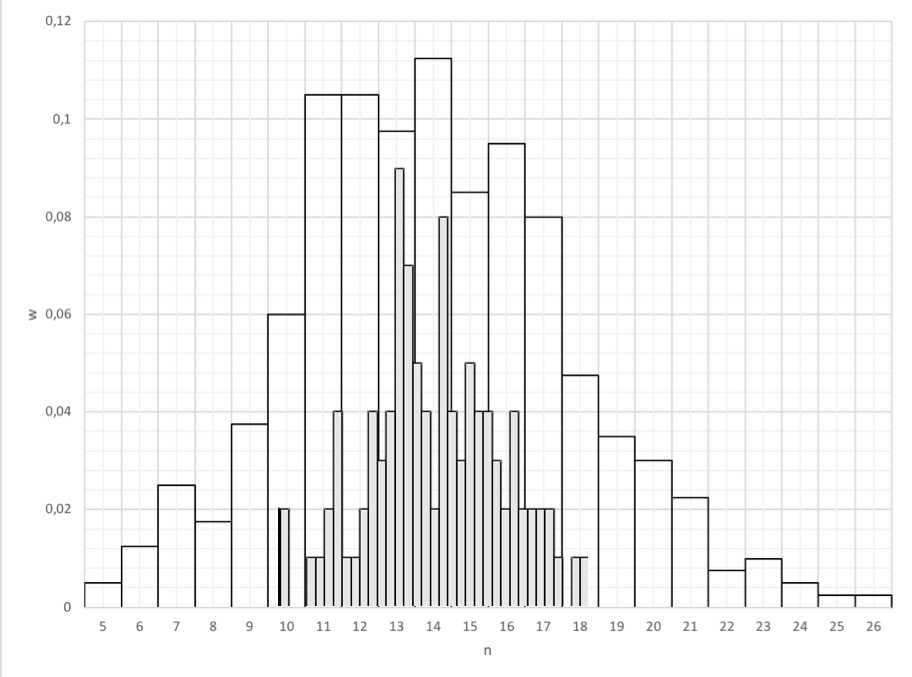
\includegraphics[width=1\textwidth]{12}
\caption{Гистограммы для $\tau = 10c$ и $\tau = 40c$}
\end{figure}
\section{Обсуждение результатов и выводы}
В результате эксперимента убеждаемся, что при увеличении числа измерений:
\begin{enumerate}
\item измеряемая величина флуктуирует
\item флуктуация среднего значения измеряемой величины уменьшается, и среднее значение выходит на постоянную величину
\item флуктуации величины погрешности отдельного измерения уменьшаются, и погрешность отдельного измерения (погрешность метода) выходит на постоянную величину
\item флуктуация величины погрешности среднего значения уменьшается, а сама величина убывает
\end{enumerate}
В работе были измерены плотности потоков космического излучения через число срабатываний счетчика за 10с и 40с соответсвенно.
\[n_{t=10c} = \overline{n}_1 \pm \sigma_{\overline{n}_1} = 14,00 \pm 0,19\]
\[n_{t=40c} = \overline{n}_2 \pm \sigma_{\overline{n}_2} = 56,00 \pm 0,74\]

Также в работе было проверено утверждение, что $\sigma_\text{отд} \approx \sqrt{\overline{n}}$. По вычислениям в работе формула оказалась верна.

Было преведено сравнение доли случаев, когда отклонение от среднего значения не превышает $\sigma_1$, $2\sigma_1$ с теоритической оценкой. Результаты измерений оказались очень близки к теоретической оценке, что свидетельствует о выполнении закона нормального распределения.

Ширина гистограммы определяется $\sigma$ (среднеквадратичной ошибкой отдельного измерения). Чем больше $\sigma$  тем больше ширина гистограммы.
\end{document}
